\chapter{Resultados}\label{cap4_resultados}

{ Após a exposição dos componentes do ambiente de aprendizado e estrutura das
    implementações do processador, é possível realizar análises quantitativas
    e qualitativas dos resultados obtidos.
}

{ As seções desse capítulo explorarão os resultados da síntese e simulação de
    cada versão, além de apresentar resultados de \textit{benchmarks} sintéticos
    a fim de comparar o desempenho de cada implementação e sua viabilidade de uso.
}

{ O código-fonte e demais arquivos da plataforma \textit{RISC-V SiMPLE} denvolvida
    está disponível no \textit{link} \url{https://github.com/LAICO-UnB/riscv-simple}
    com licença \textit{open-source BSD 3-Clause}. O código-fonte e \texttt{.pdf}
    dessa monografia está disponível no \textit{link} \url{https://github.com/arthurbeggs/monografia}
    com licença \textit{open-source BSD 3-Clause}.
}

\section{Síntese dos \textit{soft-cores}}
    { As nove diferentes implementações do processador foram geradas usando o \textit{script}
        \texttt{./make.sh \--simulate}, produzindo os arquivos \texttt{.sof} para
        gravação na \textit{FPGA}, os \texttt{.vcd} de simulação em forma de onda
        e os \texttt{.rpt} de resumo do \textit{Quartus}.
    }

    { Os dados da Tabela~\ref{table:synth_resources} foram obtidos dos arquivos
        \texttt{.rpt} e executando os arquivos \texttt{.sof} na placa \textit{DE1-SoC}.
        Cada \textit{ISA} foi carregada com um \textit{benchmark} específico para seu
        conjunto de instruções. Os códigos-fonte podem ser encontrados em
        \texttt{test/assembly\_testbench} e suas versões montadas estão disponíveis
        na pasta \texttt{test/mif\_library}.
    }

    \begin{longtable}{cc|c|c|c|c|c|c|c|}
        \caption{Características dos sistemas implementados}\label{table:synth_resources}\\
        \cline{3-9}
                                                                &                               & ALMs  & Regs  & Pins  & Mem Bits  & DSPs  & PLLs  & Max Clk   \\
        \cline{2-9}
                                                                & \multicolumn{1}{|c|}{Máximo}  & 32070 & XXXXX & 457   & 4065280   & 87    & 1     & 50MHz     \\
        \hline
        \endfirsthead
        \cline{3-9}
                                                                &                               & ALMs  & Regs  & Pins  & Mem Bits  & DSPs  & PLLs  & Max Clk   \\
        \cline{2-9}
                                                                & \multicolumn{1}{|c|}{Máximo}  & 32070 & XXXXX & 457   & 4065280   & 87    & 1     & 50MHz     \\
        \hline
        \endhead
        \multicolumn{1}{|c}{\multirow{3}{*}{{Uniciclo}}}        & \multicolumn{1}{|c|}{RV32I}   & 4123  & 3160  & 103   & 2805792   & 0     & 1     & 12.5MHz   \\*
        \cline{2-9}
        \multicolumn{1}{|c}{ }                                  & \multicolumn{1}{|c|}{RV32IM}  & 7047  & 3179  & 103   & 2805792   & 12    & 1     & 12.5MHz   \\*
        \cline{2-9}
        \multicolumn{1}{|c}{ }                                  & \multicolumn{1}{|c|}{RV32IMF} & 9411  & 5558  & 103   & 2853408   & 18    & 1     & 4.17Mhz   \\
        \hline
        \multicolumn{1}{|c}{\multirow{3}{*}{{Multiciclo}}}      & \multicolumn{1}{|c|}{RV32I}   & 4102  & 3444  & 103   & 2805792   & 0     & 1     & 25MHz     \\*
        \cline{2-9}
        \multicolumn{1}{|c}{ }                                  & \multicolumn{1}{|c|}{RV32IM}  & 6726  & 3471  & 103   & 2805792   & 12    & 1     & 25MHz     \\*
        \cline{2-9}
        \multicolumn{1}{|c}{ }                                  & \multicolumn{1}{|c|}{RV32IMF} & 9108  & 5737  & 103   & 2853408   & 18    & 1     & 25MHz     \\
        \hline
        \multicolumn{1}{|c}{\multirow{3}{*}{\textit{Pipeline}}} & \multicolumn{1}{|c|}{RV32I}   & 4605  & 4139  & 103   & 2805792   & 0     & 1     & 50MHz     \\*
        \cline{2-9}
        \multicolumn{1}{|c}{ }                                  & \multicolumn{1}{|c|}{RV32IM}  & 7376  & 4145  & 103   & 2805792   & 12    & 1     & 25MHz     \\*
        \cline{2-9}
        \multicolumn{1}{|c}{ }                                  & \multicolumn{1}{|c|}{RV32IMF} & 9750  & 6568  & 103   & 2853408   & 18    & 1     & 25MHz*    \\
        \hline
    \end{longtable}

    { Ao analisar a tabela, podemos tirar as seguintes conclusões: }
    \begin{itemize}
        \item   O número de \textit{PLLs} e de pinos não muda entre as implementações,
            pois somente um \textit{PLL} é utilizado para gerar os sinais de relógio da
            \textit{FPGA}, e o \textit{pinout} do módulo \textit{top level} não é alterado
            entre as versões do processador. Variação nesses valores representaria um erro;
        \item   O número de \textit{DSPs} é \texttt{0} para o uniciclo, \texttt{12} para o
            multiciclo e \texttt{18} para o \textit{pipeline}. Os \textit{DSPs} apenas
            são utilizados nas operações de \textit{mul/div} e ponto flutuante;
        \item   A quantia de \textit{bits} de memória utilizados permanece igual para
            todas as implementações do uniciclo e multiciclo. Todas as implementações
            do \textit{pipeline} também utilizam a mesma quantia de \textit{bits}, que
            é levemente maior que nas outras duas microarquiteturas;
        \item   Como é de se esperar, a quantia de \textit{ALMs} e \textit{registradores}
            aumenta ao implementar mais extensões numa mesma microarquitetura;
        \item   A microarquitetura multiciclo utiliza a menor quantia de recursos entre
            as três, resultado esperado já que sua implementação reutiliza estruturas como
            a ULA na sua execução por microcódigo, enquanto as outras arquiteturas utilizam
            mais de um somador com funções específicas em seu \textit{datapath};
        \item   A frequência máxima de operação do multiciclo se manteve constante para as
            três \textit{ISAs} implementadas e teve bom desempenho;
        \item   A frequência de operação do uniciclo foi a mais baixa entre os sistemas
            implementados, como era esperado. Com o uso de operações de ponto flutuante,
            sua frequência máxima foi bastante penalizada;
        \item   A implementação da \textit{ISA RV32IMF} no \textit{pipeline} apresenta
            erros devido a \textit{forwards e hazards} não tratados ou tratados de maneira
            incorreta. Há um ``*'' em sua frequência pois não é possível realizar o teste
            até sua complitude.
    \end{itemize}

\section{Formas de Onda das Simulações}
    { As Figuras \ref{fig:gtkwave_uni}, \ref{fig:gtkwave_multi} e \ref{fig:gtkwave_pipe}
        mostram as visualizações criadas para as simulações dos \textit{soft-cores}
        \textbf{RV32IMF} uniciclo, multiciclo e \textit{pipeline} respectivamente.
        Nelas, as instruções passam por um \textit{desassembler}, os registradores
        são mostrados com seus nomes mnemônicos e os sinais possuem cores diferentes
        dependendo de sua origem.
    }

    { Com essas visualizações, o processo de depuração do processador é facilitado.
        Alguns \textit{bugs} do \textit{pipeline} só puderam ser identificados graças
        à simulação. Os sinais adicionados são suficientes para a maioria das inspeções,
        mas se necessário, novos sinais podem ser adicionados.
    }

    \begin{figure}[H]
    \centering
        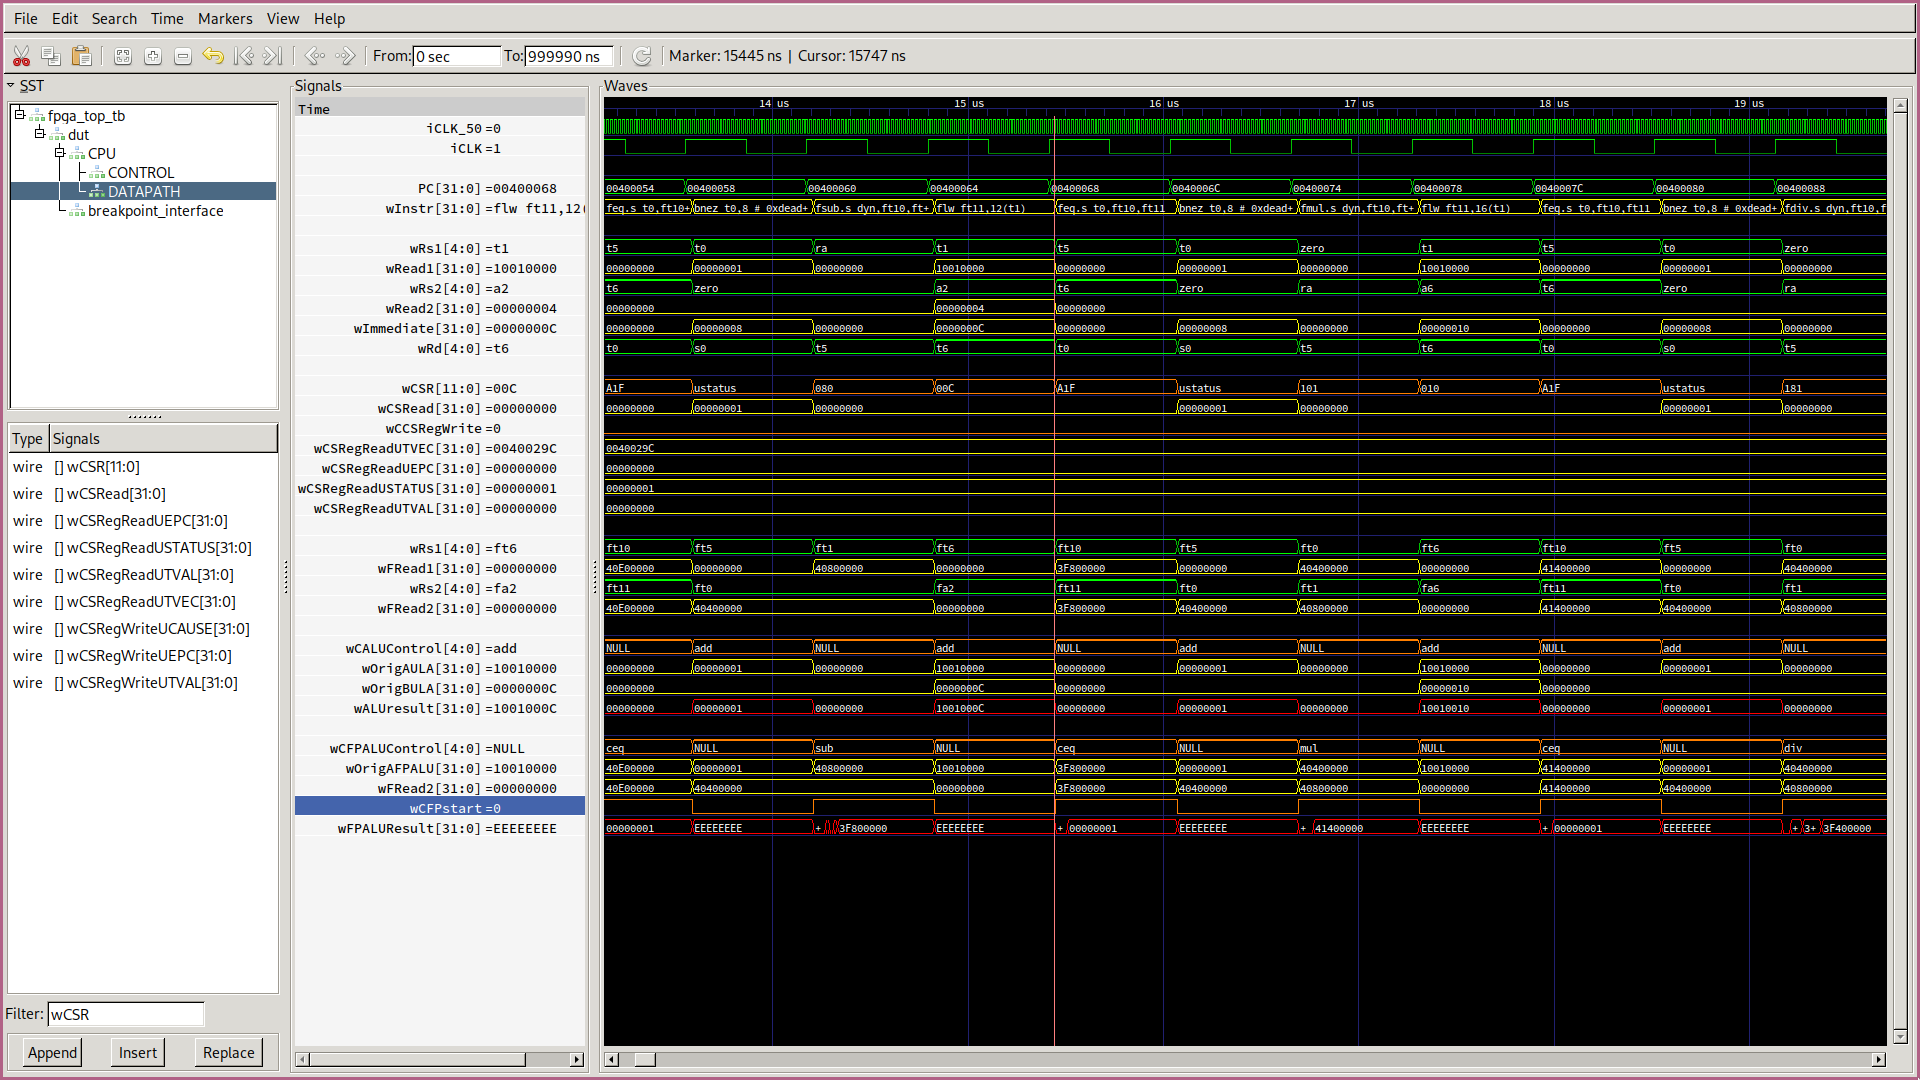
\includegraphics[width=0.9\linewidth]{../images/gtkwave/gtkwave_uni.png}
        \caption{Visualização das formas de onda \textit{soft-core} \textbf{RV32IMF} uniciclo}
        \label{fig:gtkwave_uni}
    \end{figure}

    \begin{figure}[H]
    \centering
        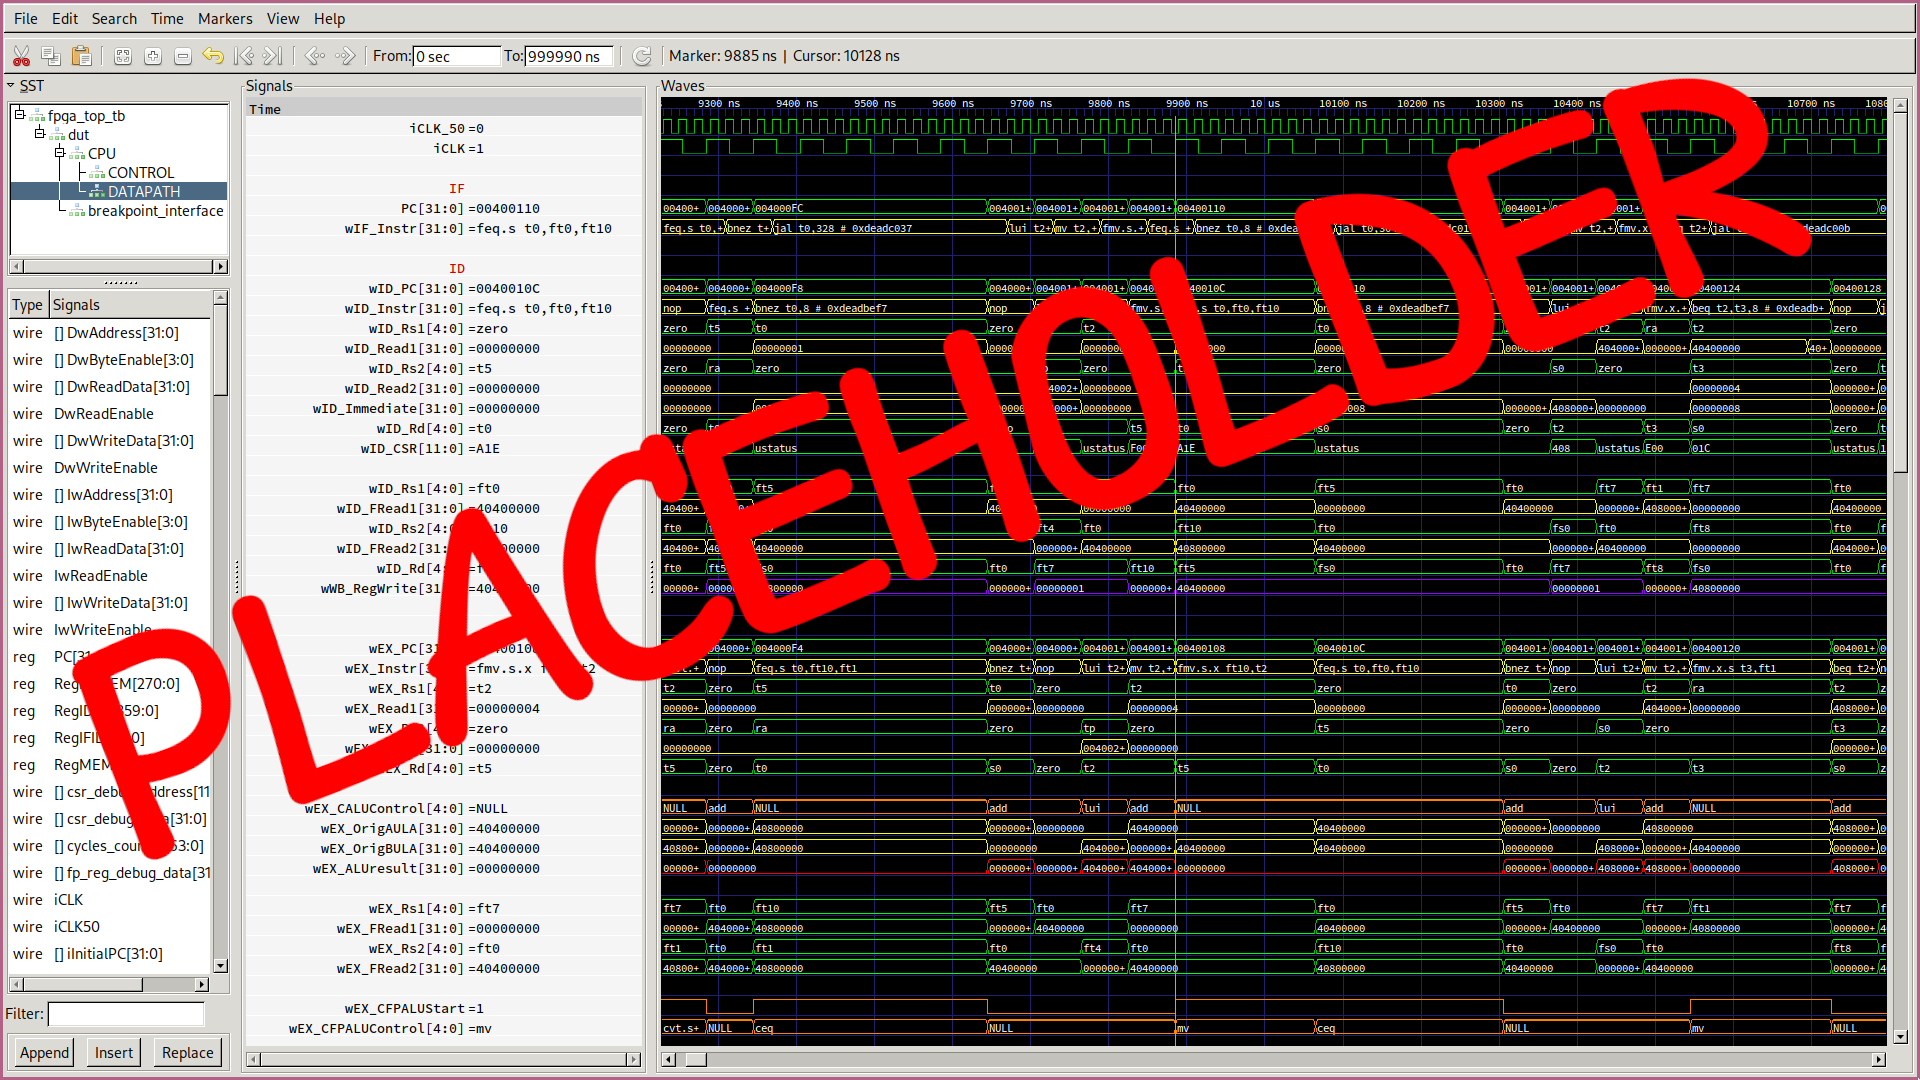
\includegraphics[width=0.9\linewidth]{../images/gtkwave/gtkwave_multi.png}
        \caption{Visualização das formas de onda \textit{soft-core} \textbf{RV32IMF} multiciclo}
        \label{fig:gtkwave_multi}
    \end{figure}

    \begin{figure}[H]
    \centering
        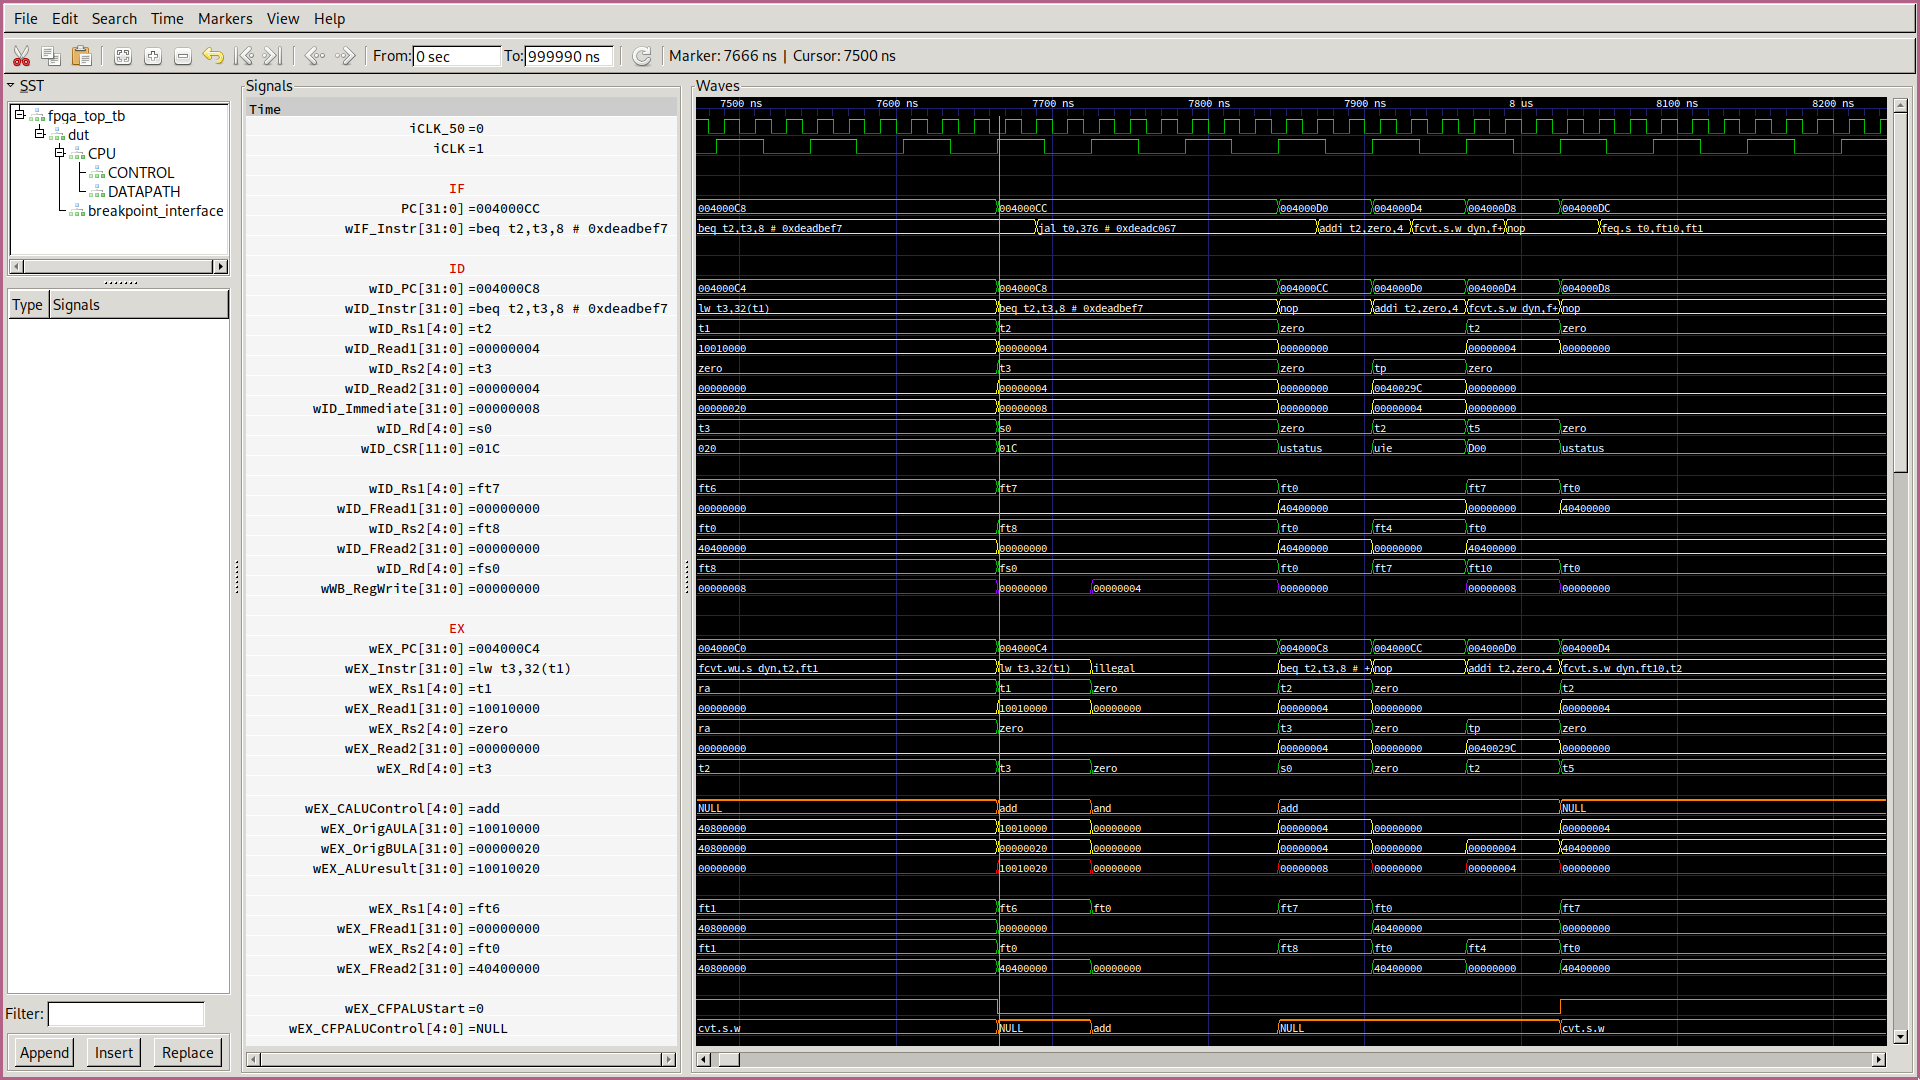
\includegraphics[width=0.9\linewidth]{../images/gtkwave/gtkwave_pipe.png}
        \caption{Visualização das formas de onda \textit{soft-core} \textbf{RV32IMF} \textit{pipeline}}
        \label{fig:gtkwave_pipe}
    \end{figure}

\section{\textit{Benchmarks} (Incompleto)}
    {
    }
    \begin{longtable}{|l|}
        \caption{\textit{Benchmark}}\label{table:benchmark}\\
        \hline
        \hline
        \endfirsthead
        \hline
        \hline
        \endhead
        \hline
    \end{longtable}

\section{Observações Finais dos Resultados (Incompleto)}
    % NOTE: Falar sobre os benchmarks

    { O próximo capítulo encerrará o presente trabalho fazendo observações
        pertinentes aos resultados obtidos, à viabilidade do uso da plataforma
        desenvolvida para os propósitos desejados e perspectivas futuras,
        tratando de possíveis melhorias e expansão do escopo.
    }

